%iffalse
\let\negmedspace\undefined
\let\negthickspace\undefined
\documentclass[journal,12pt,onecolumn]{IEEEtran}
\usepackage{cite}
\usepackage{amsmath,amssymb,amsfonts,amsthm}
\usepackage{algorithmic}
\usepackage{graphicx}
\usepackage{textcomp}
\usepackage{xcolor}
\usepackage{txfonts}
\usepackage{listings}
\usepackage{enumitem}
\usepackage{mathtools}
\usepackage{gensymb}
\usepackage{comment}
\usepackage[breaklinks=true]{hyperref}
\usepackage{tkz-euclide} 
\usepackage{gvv}                                        
%\def\inputGnumericTable{}                                 
\usepackage[latin1]{inputenc}     
\usepackage{xparse}
\usepackage{color}                                            
\usepackage{array}                                            
\usepackage{longtable}                                       
\usepackage{calc}                                             
\usepackage{multirow}
\usepackage{multicol}
\usepackage{hhline}                                           
\usepackage{ifthen}                                           
\usepackage{lscape}
\usepackage{tabularx}
\usepackage{array}
\usepackage{float}
\newtheorem{theorem}{Theorem}[section]
\newtheorem{problem}{Problem}
\newtheorem{proposition}{Proposition}[section]
\newtheorem{lemma}{Lemma}[section]
\newtheorem{corollary}[theorem]{Corollary}
\newtheorem{example}{Example}[section]
\newtheorem{definition}[problem]{Definition}
\newcommand{\BEQA}{\begin{eqnarray}}
\newcommand{\EEQA}{\end{eqnarray}}
%\newcommand{\define}{\stackrel{\triangle}{=}}
\theoremstyle{remark}
%\newtheorem{rem}{Remark}
% Marks the beginning of the document
\begin{document}
\title{gate 1}
\author{AI25btech11033-Spoorthi N}
\maketitle
\renewcommand{\thefigure}{\theenumi}
\renewcommand{\thetable}{\theenumi}
\begin {center}
\large \textbf{2020}\\
\large \textbf{STATISTICS}\\

\end{center}

\begin{center}
\textbf{ST: Statistics}\\[6pt]
\textbf{GA - General Aptitude}\\[6pt]
\textbf{Q1 - Q5 carry one mark each.}
\end{center}

\begin{enumerate}

\item Rajiv Gandhi Khel Ratna Award was conferred \_\_\_\_ Mary Kom, a six-time world 
champion in boxing, recently in a ceremony \_\_\_\_ the Rashtrapati Bhawan (the President's 
official residence) in New Delhi. \hfill \textbf{(GATE EE 2025)}

\begin{enumerate}
\item with, at 
\item on, in 
\item on, at 
\item to, at
\end{enumerate}


\item Despite a string of poor performances, the chances of K. L. Rahul's selection in the team are 
\_\_\_\_\_ \hfill \textbf{(GATE EE 2025)}
\begin{enumerate}
\item slim 
\item bright 
\item obvious 
\item uncertain
\end{enumerate}


\item Select the word that fits the analogy: \\ 
\textbf{Cover : Uncover :: Associate : \_\_\_\_} \hfill \textbf{(GATE EE 2025)}

\begin{enumerate}
\item Unassociate 
\item Inassociate 
\item Misassociate 
\item Dissociate
\end{enumerate}

\item Hit by floods, the kharif (summer sown) crops in various parts of the country have been affected. Officials believe that the loss in production of the kharif crops can be recovered in the output of the rabi (winter sown) crops so that the country can achieve its food-grain production target of 291 million tons in the crop year 2019-20 (July-June). They are hopeful that good rains in July-August will help the soil retain moisture for a longer period, helping winter sown crops such as wheat and pulses during the November-February period. 
Which of the following statements can be inferred from the given passage?
\hfill \textbf{(GATE EE 2025)}
\begin{enumerate}
\item Officials declared that the food-grain production target will be met due to good rains. 
\item Officials want the food-grain production target to be met by the November to February period. 
\item Officials feel that the food-grain production target cannot be met due to floods. 
\item Officials hope that the food-grain production target will be met due to a good rabi produce.
\end{enumerate}


\item The difference between the sum of the first $2n$ natural numbers and the sum of the first $n$ odd natural numbers is \_\_\_\_. \hfill \textbf{(GATE EE 2025)}

\begin{enumerate}
\item $n^2 - n$ 
\item $n^2 + n$ 
\item $2n^2 - n$ 
\item $2n^2 + n$
\end{enumerate}


\textbf{Q6 -- Q10 carry two marks each.}

\item Repo rate is the rate at which Reserve Bank of India (RBI) lends commercial banks, and reverse repo rate is the rate at which RBI borrows money from commercial banks. 

Which of the following statements can be inferred from the above passage? \\ \hfill \textbf{(GATE EE 2025)}
\begin{enumerate}
\item Decrease in repo rate will increase cost of borrowing and decrease lending by commercial banks.
\item Increase in repo rate will decrease cost of borrowing and increase lending by commercial banks.
\item Increase in repo rate will decrease cost of borrowing and decrease lending by commercial banks.
\item Decrease in repo rate will decrease cost of borrowing and increase lending by commercial banks.
\end{enumerate}


\item P, Q, R, S, T, U, V, and W are seated around a circular table. \\
I. S is seated opposite to W. \\
II. U is seated at the second place to the right of R. \\
III. T is seated at the third place to the left of R. \\
IV. V is a neighbour of S. \\

Which of the following must be true? \\ \hfill \textbf{(GATE EE 2025)}
\begin{enumerate}
\item P is a neighbour of R.
\item Q is a neighbour of R.
\item P is not seated opposite to Q.
\item R is the left neighbour of S.
\end{enumerate}


\item The distance between Delhi and Agra is 233 km. A car \textit{P} started travelling from Delhi to Agra and another car \textit{Q} started from Agra to Delhi along the same road 1 hour after the car \textit{P} started. The two cars crossed each other 75 minutes after the car \textit{Q} started. Both cars were travelling at constant speed. The speed of car \textit{P} was 10 km/hr more than the speed of car \textit{Q}. How many kilometers the car \textit{Q} had travelled when the cars crossed each other? \\
\hfill \textbf{(GATE EE 2025)}
\begin{enumerate}
\item 66.6
\item 75.2
\item 88.2
\item 116.5
\end{enumerate}


\item For a matrix $M = [m_{ij}], \, i,j = 1,2,3,4$, the diagonal elements are all zero and $m_{ij} = -m_{ji}$. The minimum number of elements required to fully specify the matrix is \_\_\_. \\
\hfill \textbf{(GATE EE 2025)}
\begin{enumerate}
\item 0
\item 6
\item 12
\item 16
\end{enumerate}
\item The profit shares of two companies P and Q are shown in the figure. 
If the two companies have invested a fixed and equal amount every year, then the ratio of the total revenue of company P to the total revenue of company Q, during 2013 -- 2018 is \_\_\_.\hfill \textbf{(GATE EE 2025)}
\begin{figure}[H]
    \centering
    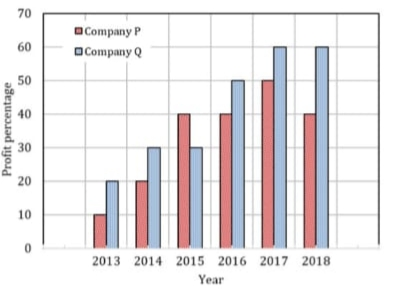
\includegraphics[width=0.5\linewidth]{fig10.png}
    \caption{}
    \label{fig10}
\end{figure}
\begin{enumerate}
\item  15 : 17 \item   16 : 17 \item   17 : 15 \item  17 : 16
\end{enumerate}

\item Let $M$ be a $3 \times 3$ non-zero idempotent matrix and let $I_3$ denote the $3 \times 3$ identity matrix. Then which of the following statements is \textbf{FALSE}? \hfill \textbf{(GATE EE 2025)}
\begin{enumerate}
    \item The eigenvalues of $M$ are $0$ and $1$
    \item $\text{Rank}(M) = \text{Trace}(M)$
    \item $I_3 - M$ is idempotent
    \item $(I_3 + M)^{-1} = I_3 - 2M$
\end{enumerate}
\item Let $\mathbb{C}$ denote the set of all complex numbers. Consider the vector space \hfill \textbf{(GATE EE 2025)}
\[
V = \{(a,b,c) : a,b,c \in \mathbb{C}, \; a + \bar{b} = 0, \; b + \bar{c} = 0 \},
\]
over the field of real numbers, where for any complex number $z$, $\bar{z}$ denotes its complex conjugate. If $i = \sqrt{-1}$, then a basis of $V$ is
\begin{enumerate}
    \item $\{(1,-1,1), \; (i,i,i)\}$
    \item $\{(1,-1,1), \; (i,-i,i)\}$
    \item $\{(1,-i,1), \; (i,1,i)\}$
    \item $\{(1,-i,1), \; (i,1,-i)\}$
\end{enumerate}

\item Let 
\[
S = \{(x,y) \in \mathbb{R} \times \mathbb{R} : x^2 - y^2 = 4 \}
\]
and $f : S \to \mathbb{R}$ be defined by \hfill \textbf{(GATE EE 2025)}
\[
f(x,y) = 6x + y^2,
\]
where $\mathbb{R}$ denotes the set of all real numbers. Then $f$ is bounded on $S$.
\begin{enumerate} 
    \item The maximum value of $f$ on $S$ is $13$
    \item The minimum value of $f$ on $S$ is $-14$
    \item The minimum value of $f$ on $S$ is $-13$
    \item The minimum value of $f$ on $S$ is $-12$
\end{enumerate}

\item Let $f:\mathbb{R} \times \mathbb{R} \to \mathbb{R}$ be defined by. \hfill \textbf{(GATE EE 2025)}
\[
f(x,y) =
\begin{cases}
\dfrac{4x^{2} + 9y^{2}}{\sqrt{4x^{2} + 9y^{2} + 64} - 8}, & (x,y) \neq (0,0), \\[1em]
c, & (x,y) = (0,0),
\end{cases}
\]
where $\mathbb{R}$ denotes the set of all real numbers and $c \in \mathbb{R}$ is a fixed constant. Then, which of the following statements is TRUE?

\begin{enumerate}
\item There does \textbf{NOT} exist a value of $c$ for which $f$ is continuous at $(0,0)$
\item $f$ is continuous at $(0,0)$ if $c = 0$
\item $f$ is continuous at $(0,0)$ if $c = 10$
\item $f$ is continuous at $(0,0)$ if $c = 16$
\end{enumerate}

\item The moment generating function of a random variable $X$ is given by. \hfill \textbf{(GATE EE 2025)}
\[
M_X(t) = \frac{1}{6} + \frac{1}{3}e^t + \frac{1}{3}e^{2t} + \frac{1}{6}e^{3t}, \quad -\infty < t < \infty.
\]
Then $P(X \leq 2)$ equals
\[
\begin{array}{ll}
\text{(A)} & \tfrac{1}{3} \\[6pt]
\text{(B)} & \tfrac{1}{6} \\[6pt]
\text{(C)} & \tfrac{1}{2} \\[6pt]
\text{(D)} & \tfrac{5}{6} \\
\end{array}
\]


\item Consider the following two-way fixed effects analysis of variance model. \hfill \textbf{(GATE EE 2025)}
\[
Y_{ijk} = \mu + \alpha_i + \beta_j + \epsilon_{ijk}, \quad i = 1,2; \ j=1,2,3; \ k=1,2,3,
\]
where $\epsilon_{ijk}$'s are independently and identically distributed $N(0, \sigma^2)$ random variables, 
$\sigma \in (0,\infty)$, $\alpha_1 + \alpha_2 = 0$ and $\beta_1 + \beta_2 + \beta_3 = 0$. Let $SSE$ denote the sum of squares due to error. For any positive integer $\nu$ and any $\alpha \in (0,1)$, let $\chi^2_{\nu,\alpha}$ denote the $(1-\alpha)$-th quantile of the central chi-square distribution with $\nu$ degrees of freedom. Then a 95\% confidence interval for $\sigma^2$ is given by
\[
\begin{array}{ll}
\text{(A)} & \left(0, \dfrac{SSE}{\chi^2_{13,0.95}}\right) \\[12pt]
\text{(B)} & \left(0, \dfrac{SSE}{\chi^2_{13,0.05}}\right) \\[12pt]
\text{(C)} & \left(0, \dfrac{SSE}{\chi^2_{14,0.05}}\right) \\[12pt]
\text{(D)} & \left(0, \dfrac{SSE}{\chi^2_{14,0.95}}\right) \\
\end{array}
\]


\item Let $X_{1}, \ldots, X_{20}$ be independent and identically distributed random variables with the common probability density function .\hfill \textbf{(GATE EE 2025)}

\[
f(x) = \frac{1}{6} e^{-\frac{|x-2|}{3}}, \quad x \in (-\infty, \infty).
\]

Then the distribution of the random variable  

\[
W = \frac{2}{3} \sum_{i=1}^{20} |X_i - 2|
\]

is  

\begin{enumerate}
    \item central chi-square with 10 degrees of freedom
    \item central chi-square with 20 degrees of freedom
    \item central chi-square with 30 degrees of freedom
    \item central chi-square with 40 degrees of freedom
\end{enumerate}


\item Let $X_{1}, \ldots, X_{10}$ be a random sample from a Weibull distribution with the probability density function
\[
f(x;\theta) = 
\begin{cases}
3 \theta x^{2} e^{-\theta x^{3}}, & x > 0 \\
0, & \text{otherwise}
\end{cases}
\]
where $\theta \in (0, \infty)$. For any positive integer $v$ and any $\alpha \in (0,1)$, let $\chi^2_{v, \alpha}$ denote the $(1-\alpha)$-th quantile of the central chi-square distribution with $v$ degrees of freedom. Then, a 90\% confidence interval for $\theta$ is.\hfill \textbf{(GATE EE 2025)}
\[
\text{(A)} \quad \left( \frac{\chi^2_{20,0.95}}{2 \sum_{i=1}^{10} X_i^3}, \ \frac{\chi^2_{20,0.05}}{2 \sum_{i=1}^{10} X_i^3} \right)
\]
\[
\text{(B)} \quad \left( \frac{\chi^2_{10,0.95}}{2 \sum_{i=1}^{10} X_i^3}, \ \frac{\chi^2_{10,0.05}}{2 \sum_{i=1}^{10} X_i^3} \right)
\]
\[
\text{(C)} \quad \left( \frac{\chi^2_{20,0.95}}{3 \sum_{i=1}^{10} X_i^3}, \ \frac{\chi^2_{20,0.05}}{3 \sum_{i=1}^{10} X_i^3} \right)
\]
\[
\text{(D)} \quad \left( \frac{\chi^2_{10,0.95}}{3 \sum_{i=1}^{10} X_i^3}, \ \frac{\chi^2_{10,0.05}}{3 \sum_{i=1}^{10} X_i^3} \right)
\]


\item Let $X_{1}, \ldots, X_{n}$ be a random sample of size $n \ (\geq 2)$ from a uniform distribution on the interval $[-\theta, \theta]$, where $\theta \in (0, \infty)$. A minimal sufficient statistic for $\theta$ is.\hfill \textbf{(GATE EE 2025)}
\[
\text{(A)} \quad \max_{1 \leq i \leq n} X_i
\]
\[
\text{(B)} \quad \left( -\min_{1 \leq i \leq n} X_i, \ \max_{1 \leq i \leq n} X_i \right)
\]
\[
\text{(C)} \quad \max_{1 \leq i \leq n} |X_i|
\]
\[
\text{(D)} \quad \min_{1 \leq i \leq n} |X_i|
\]


\item Let $X_{1}, \ldots, X_{n}$ be a random sample of size $n \ (\geq 2)$ from $N(\theta, 2\theta^2)$ distribution, where $\theta \in (0, \infty)$. Which of the following statements is TRUE? \hfill \textbf{(GATE EE 2025)}
\[
\text{(A)} \quad \frac{1}{n(n+2)} \Big(\sum_{i=1}^n X_i \Big)^2 \ \text{is the unique unbiased estimator of } \theta^2 \text{ that is a function of minimal sufficient statistic}
\]
\[
\text{(B)} \quad \frac{1}{(3n+1)} \sum_{i=1}^n X_i^2 \ \text{is an unbiased estimator of } \theta^2
\]
\[
\text{(C)} \quad \text{There exist infinite number of unbiased estimators of } \theta^2 \text{ which are functions of minimal sufficient statistic}
\]
\[
\text{(D)} \quad \text{There does NOT exist any unbiased estimator of } \theta(\theta+1) \text{ that is a function of minimal sufficient statistic}
\]


\item Let $\{N(t), \ t \geq 0\}$ be a Poisson process with rate $\lambda = 2$. Given that $N(3) = 1$, the expected arrival time of the first event of the process is.\hfill \textbf{(GATE EE 2025)}
\begin{enumerate}
    \item 1
    \item 2
    \item $\frac{3}{2}$
    \item 3
\end{enumerate}


\item Consider the regression model.\hfill \textbf{(GATE EE 2025)}
\[
Y_i = \beta_0 + \beta_1 x_i^2 + \epsilon_i, \quad i=1,2,\ldots,n \quad (n \geq 2);
\]
where $\beta_0$ and $\beta_1$ are unknown parameters and $\epsilon_i$'s are random errors.  
Let $y_i$ be the observed value of $Y_i$, $i=1,\ldots,n$. Using the method of ordinary least squares, the estimate of $\beta_1$ is

\[
\text{(A)} \quad \frac{\tfrac{1}{n}\left(n \sum x_i^2 y_i - (\sum y_i)(\sum x_i^2)\right)}{\sum x_i^4 - \tfrac{1}{n}(\sum x_i^2)^2}
\]

\[
\text{(B)} \quad \frac{n \sum x_i^2 y_i - (\sum y_i)(\sum x_i^2)}{n \sum x_i^4 - (\sum x_i^2)^2}
\]

\[
\text{(C)} \quad \frac{\sum x_i^2 y_i - (\sum y_i)(\sum x_i^2)}{\sum x_i^4 - (\sum x_i^2)^2}
\]

\[
\text{(D)} \quad \frac{\sum x_i^2 y_i - n(\sum y_i)(\sum x_i^2)}{\sum x_i^4 - n(\sum x_i^2)^2}
\]

\item Let $X_1, \ldots, X_n$ be a random sample of size $n (\geq 2)$ from $N_p(0,\Sigma)$ distribution, where $1 \leq p \leq n-1$ and $\Sigma$ is a positive definite matrix. Define
\[
\bar{X} = \frac{1}{n} \sum_{i=1}^n X_i 
\quad \text{and} \quad 
(n-1)S = \sum_{i=1}^n (X_i - \bar{X})(X_i - \bar{X})'.
\]

Then the distribution of the statistic \hfill \textbf{(GATE EE 2025)}
\[
T^2 = n \, \bar{X}' S^{-1} \bar{X}
\]

is

\[
\text{(A)} \quad \chi_p^2, \ \text{the central chi-square distribution with $p$ degrees of freedom}
\]

\[
\text{(B)} \quad F_{p,n-p}, \ \text{the central $F$ distribution with $p$ and $n-p$ degrees of freedom}
\]

\[
\text{(C)} \quad \frac{n(n-1)}{n-p} F_{p,n-p}, \ \text{where $F_{p,n-p}$ is the central $F$ distribution with $p$ and $n-p$ degrees of freedom}
\]

\[
\text{(D)} \quad \frac{n-p}{(n-1)p} F_{n-p,p}, \ \text{where $F_{n-p,p}$ is the central $F$ distribution with $n-p$ and $p$ degrees of freedom}
\]


\item Consider a two-way fixed effects analysis of variance model without interaction effect and one observation per cell. If there are 5 factors and 4 columns, then the degrees of freedom for the error sum of squares is \hfill \textbf{(GATE EE 2025)}

\[
\text{(A) } 20 \quad \text{(B) } 19  \quad\text{(C) } 12 \text {(D) } 11
\]

\item Let $X_1, \ldots, X_n$ be a random sample of size $n (\geq 2)$ from an exponential distribution with the probability density function \hfill \textbf{(GATE EE 2025)}
\[
f(x;\theta) = 
\begin{cases}
\frac{1}{\theta} e^{-x/\theta}, & x > 0, \\
0, & \text{otherwise,}
\end{cases}
\]
where $\theta \in \{1,2\}$. Consider the problem of testing $H_0: \theta=1$ against $H_1: \theta=2$, based on $X_1, \ldots, X_n$. Which of the following statements is TRUE? 

\[
\text{(A)} \quad \text{Likelihood ratio test at level $\alpha \ (0 < \alpha < 1)$ leads to the same critical region as the corresponding most powerful test at the same level.}
\]

\[
\text{(B)} \quad \text{Critical region of level $\alpha \ (0 < \alpha < 1)$ likelihood ratio test is } 
\{(x_1,\ldots,x_n): \sum_{i=1}^n x_i < 0.5 \, \chi^2_{2n,1-\alpha}\},
\]
where $\chi^2_{2n,1-\alpha}$ is the $\alpha$-th quantile of the central chi-square distribution with $2n$ degrees of freedom.


\[
\text{(C)} \quad \text{Likelihood ratio test for testing $H_0$ against $H_1$ does not exist.}
\]

\[
\text{(D)} \quad \text{At any fixed level $\alpha \ (0 < \alpha < 1)$, the power of the likelihood ratio test is lower than that of the most powerful test.}
\]

  
 \item The characteristic function of a random variable $X$ is given by \hfill \textbf{(GATE EE 2025)}
    \[
        \phi_X(t) = 
        \begin{cases}
            \dfrac{\sin t \cos t}{t}, & \text{for } t \neq 0, \\
            1, & \text{for } t = 0
        \end{cases}
    \]
    Then \[
        P\left( |X| \leq \tfrac{3}{2} \right) = \_\_\_\_\_\_ 
        \quad (\text{correct up to two decimal places}).
    \]
\item Let the random vector $X = (X_1, X_2, X_3, X_4)$ follow $N_4(\mu, \Sigma)$ distribution, where
\hfill \textbf{(GATE EE 2025)}
    \[
        \mu = 
        \begin{bmatrix}
            
        \end{bmatrix}
            0 \\ 0 \\ 0 \\ 0
        end{bmatrix}
        \quad 
        \Sigma = 
        \begin{bmatrix}
            1   & 0.7 & 0.6 & 0.4 \\
            0.7 & 1   & 0.5 & 0.8 \\
            0.6 & 0.5 & 1   & 0.7 \\
            0.4 & 0.8 & 0.7 & 1
        \end{bmatrix}
    \]
    Then
    \[
        P(X_1 + X_2 + X_3 + X_4 > 0) = \_\_\_\_\_\_
        \quad (\text{correct up to one decimal place}).
    \]

    \item Let $\{X_n\}_{n \geq 0}$ be a homogeneous Markov chain with state space $\{0,1\}$ and one-step transition probability matrix \hfill \textbf{(GATE EE 2025)}
    \[
        P = \begin{bmatrix}
            \tfrac{1}{2} & \tfrac{1}{2} \\
            \tfrac{1}{3} & \tfrac{2}{3}
        \end{bmatrix}.
    \]
    If $P(X_0 = 0) = \tfrac{1}{3}$, then
    \[
        27 \times E(X_2) = \_\_\_\_\_\_
        \quad (\text{correct up to two decimal places}).
    \]

    % Q. No. 19
    \item Let $E, F$ and $G$ be mutually independent events with \hfill \textbf{(GATE EE 2025)}
    \[
        P(E) = \tfrac{1}{2}, \quad P(F) = \tfrac{1}{3}, \quad P(G) = \tfrac{1}{4}.
    \]
    Let $p$ be the probability that at least two of the events among $E, F$ and $G$ occur. Then
    \[
        12 \times p = \_\_\_\_\_\_
        \quad (\text{correct up to one decimal place}).
    \]

    \item Let the joint probability mass function of $(X,Y,Z)$ be \hfill \textbf{(GATE EE 2025)}
    \[
        P(X = x, Y = y, Z = z) = \frac{10!}{x! \, y! \, z! \, k!} (0.2)^x (0.3)^y (0.4)^z (0.1)^k,
    \]
    where $k = 10 - x - y - z$; $x,y,z = 0,1,\ldots,10$; $x+y+z \leq 10$.

    Then the variance of the random variable $Y+Z$ equals \_\_\_\_\_\_ 
    \quad (correct up to one decimal place).

    \item The total number of standard $4 \times 4$ Latin squares is \_\_\_\_\_\_.
    \hfill \textbf{(GATE EE 2025)}
    \item Let $X$ be a $4 \times 1$ random vector with $E(X) = 0$ and variance-covariance matrix
    \hfill \textbf{(GATE EE 2025)}
    \[
        \Sigma = 
        \begin{bmatrix}
            1 & 0.5 & 0.5 & 0.5 \\
            0.5 & 1 & 0.5 & 0.5 \\
            0.5 & 0.5 & 1 & 0.5 \\
            0.5 & 0.5 & 0.5 & 1
        \end{bmatrix}.
    \]
   \item  Let $Y$ be the $4 \times 1$ random vector of principal components derived from $\Sigma$. The proportion of total variation explained by the first two principal components equals \_\_\_\_\_\_ \quad (correct up to two decimal places).\hfill \textbf{(GATE EE 2025)}

\item Let $X_1, \ldots, X_n$ be a random sample of size $n \ (\geq 2)$ from an exponential distribution with the probability density function \hfill \textbf{(GATE EE 2025)}
\[
f(x; \theta) = \begin{cases} 
e^{-(x-2\theta)}, & x > 2\theta, \\
0, & \text{otherwise,}
\end{cases}
\]
where $\theta \in (0,\infty)$. If $X_{(1)} = \min(X_1, \ldots, X_n)$ then the conditional expectation
\[
E\!\left[\frac{1}{\theta}\left(X_{(1)} - \frac{1}{n}\right) \Big| \ X_1 - X_2 = 2 \right] = \underline{\hspace{2cm}}
\]

\item Let $Y_i = \alpha + \beta x_i + \epsilon_i, \ i=1,2,\ldots,7$, where $x-i$'s are fixed covariates and $\epsilon$ is are independent and identically distributed random variables with mean zero and finite variance. Suppose that $\alpha$ and $\beta$ are the least squares estimators of $\alpha$ and $\beta$, respectively. Given the following data: \hfill \textbf{(GATE EE 2025)}

$\sum_{i=1}^7 x_i = 0, \quad \sum_{i=1}^7 x_i^2 = 28, \quad \sum_{i=1}^7 x_i y_i = 28, \quad \sum_{i=1}^7 y_i = 21, \quad \sum_{i=1}^7 y_i^2 = 91,$

where $y_i$ is the observed value of $Y_i, \ i=1,\ldots,7$. Then the correlation coefficient between $\alpha$ and $\beta$ equals \underline{\hspace{2cm}}

\item Let $\{0,1,2,3\}$ be an observed sample of size $4$ from $N(\theta,5)$ distribution, where $\theta \in [2,\infty)$. Then the maximum likelihood estimate of $\theta$ based on the observed sample is \underline{\hspace{2cm}} \hfill \textbf{(GATE EE 2025)}


\item  $f:\mathbb{R}\times \mathbb{R} \to \mathbb{R}$ be defined by \hfill \textbf{(GATE EE 2025)}
\[
f(x,y) = x^4 - 2x^2y^3 + 16y + 17,
\]
where $\mathbb{R}$ denotes the set of all real numbers. Then 
\begin{enumerate}
    \item $f$ has a local minimum at $(2,\tfrac{4}{3})$
    \item $f$ has a local maximum at $(2,\tfrac{4}{3})$
    \item $f$ has a saddle point at $(2,\tfrac{4}{3})$
    \item $f$ is bounded
\end{enumerate}

\item Consider the linear transformation $T: \mathbb{C}^3 \to \mathbb{C}^3$ defined by \hfill \textbf{(GATE EE 2025)}
\[
T(x,y,z) = \left(x, \ \frac{\sqrt{3}}{2}y - \frac{1}{2}z, \ \frac{1}{2}y + \frac{\sqrt{3}}{2}z\right),
\]
where $\mathbb{C}$ is the set of all complex numbers and $\mathbb{C}^3 = \mathbb{C}\times \mathbb{C}\times \mathbb{C}$. Which of the following statements is TRUE?
\begin{enumerate}
    \item There exists a non-zero vector $X$ such that $T(X) = -X$
    \item There exist a non-zero vector $Y$ and a real number $\lambda \neq 1$ such that $T(Y) = \lambda Y$
    \item $T$ is diagonalizable
    \item $T^2 = I_3$, where $I_3$ is the $3 \times 3$ identity matrix
\end{enumerate}

\item For real numbers $a, b, c$, let \hfill \textbf{(GATE EE 2025)}

M = \myvec{
a & ac & 0 \\
1 & c  & 0 \\
b & bc & 1}


Then, which of the following statements is \textbf{TRUE}?
\begin{enumerate}
\item $\text{Rank}(M) = 3$ for every $a,b,c \in \mathbb{R}$
\item If $a+c=0$ then $M$ is diagonalizable for every $b \in \mathbb{R}$
\item $M$ has a pair of orthogonal eigenvectors for every $a,b,c \in \mathbb{R}$
\item If $b=0$ and $a+c=1$ then $M$ is \textbf{NOT} idempotent
\end{enumerate}


\item Let $M$ be a $4 \times 4$ matrix with $(x-1)^2(x-3)^2$ as its minimal polynomial. Then, which of the following statements is \textbf{FALSE}?
\begin{enumerate}
\item The eigenvalues of $M$ are $1$ and $3$
\item The algebraic multiplicity of the eigenvalue $1$ is $3$
\item $M$ is \textbf{NOT} diagonalizable
\item $\text{Trace}(M) = 8$
\end{enumerate}


\item Let $f : \mathbb{R} \times \mathbb{R} \to \mathbb{R}$ be defined by \hfill \textbf{(GATE EE 2025)}
\[
f(x,y) = |y - 2| \, |x - 1|, \quad (x,y) \in \mathbb{R} \times \mathbb{R},
\]
where $\mathbb{R}$ denotes the set of all real numbers. Then which of the following statements is \textbf{TRUE}?
\begin{enumerate}
\item $f$ is differentiable at $(1,2)$
\item $f$ is continuous at $(1,2)$ but \textbf{NOT} differentiable at $(1,2)$
\item The partial derivative of $f$, with respect to $x$, at $(1,2)$ does \textbf{NOT} exist
\item The directional derivative of $f$ at $(1,2)$ along $\vec{u} = \left(\tfrac{1}{\sqrt{2}}, \tfrac{1}{\sqrt{2}} \right)$ equals $1$
\end{enumerate}


\item Which of the following functions is uniformly continuous on the specified domain?
\hfill \textbf{(GATE EE 2025)}
\begin{enumerate}
\item $f_1(x) = e^{x^2}, \quad -\infty < x < \infty$
\item 
$f_2(x) = \begin{cases}
\dfrac{1}{x}, & 0 < x \leq 1 \\
0, & x=0
\end{cases}$
\item 
$f_3(x) = \begin{cases}
x^2, & |x| \leq 1 \\
\dfrac{2}{1+x^2}, & |x| > 1
\end{cases}$
\item 
$f_4(x) = \begin{cases}
x, & |x| \leq 1 \\
|x|, & |x| > 1
\end{cases}$
\end{enumerate}

\item Let the random vector $X = (X_1, X_2, X_3)$ have the joint probability density function \hfill \textbf{(GATE EE 2025)}
\[
f_X(x_1, x_2, x_3) = 
\begin{cases}
\dfrac{1 - \sin x_1 \sin x_2 \sin x_3}{8\pi^3}, & 0 \leq x_1, x_2, x_3 \leq 2\pi, \\
0, & \text{otherwise}.
\end{cases}
\]
Which of the following statements is \textbf{TRUE}?
\begin{enumerate}
\item $X_1, X_2, X_3$ are mutually independent
\item $X_1, X_2, X_3$ are pairwise independent
\item $(X_1, X_2)$ and $X_3$ are independent
\item Variance of $X_1 + X_2$ is $\pi^2$
\end{enumerate}

\item Suppose that $P_{1}$ and $P_{2}$ are two populations having bivariate normal 
distributions with mean vectors  
\myvec{
0 \\ 0
}
\quad \text{and} \quad
\myvec{
1 \\ 1
}

respectively, and the same variance-covariance matrix \hfill \textbf{(GATE EE 2025)}

\myvec{
1 & 0.5 \\
0.5 & 1
}

Let 
Z{1} =\myvec{ 0.75 \\ 0.75 }
\quad 
Z{2} = \myvec{ 0.25 \\ 0.25}

be two new observations. If the prior probabilities for $P_{1}$ and $P_{2}$ are assumed to be equal and the misclassification costs are also assumed to be equal, then, according to the linear discriminant rule, 

\begin{enumerate}
\item $Z_{1}$ is assigned to $P_{1}$ and $Z_{2}$ is assigned to $P_{2}$
\item $Z_{1}$ is assigned to $P_{2}$ and $Z_{2}$ is assigned to $P_{1}$
\item both $Z_{1}$ and $Z_{2}$ are assigned to $P_{1}$
\item both $Z_{1}$ and $Z_{2}$ are assigned to $P_{2}$
\end{enumerate}

\item Let $X_1, \ldots, X_n$ be a random sample of size $n \ (\geq 2)$ from an exponential distribution with the probability density function \hfill \textbf{(GATE EE 2025)}
\[
f(x;\theta) = 
\begin{cases}
\frac{1}{\theta} e^{-(x-\theta)/\theta}, & x > \theta, \\
0, & \text{otherwise},
\end{cases}
\]
where $\theta \in (0, \infty)$. Which of the following statements is TRUE?

\begin{enumerate}
    \item $\min\limits {1 \leq i \leq n} X_i$ is a minimal sufficient statistic
    \item $\sum\limits {i=1}^n X_i$ is a minimal sufficient statistic
    \item Any minimal sufficient statistic is complete
    \item $\left( \min\limits_{1 \leq i \leq n} X_i , \frac{1}{n} \sum\limits_{i=1}^n X_i \right)$ is minimal sufficient statistic
\end{enumerate}

\item Let the joint distribution of $(X,Y)$ be bivariate normal with mean vector \myvec{0 \\ 0 } and variance-covariance matrix 
\myvec{
1 & \rho \\
\rho & 1
} \quad -1 < ,< 1.

Then $\mathbb{E}[\max(X,Y)]$ equals: \hfill \textbf{(GATE EE 2025)}

\begin{enumerate}
    \item $\dfrac{\sqrt{1-\rho}}{\pi}$
    \item $\dfrac{\sqrt{1-\rho}}{\sqrt{\pi}}$
    \item $0$
    \item $\dfrac{1}{2}$
\end{enumerate}

\item Let $X_1, X_2, \ldots, X_{10}$ be independent and identically distributed $N_3(0, I_3)$ random vectors, where $I_3$ is the $3 \times 3$ identity matrix. Let \hfill \textbf{(GATE EE 2025)}
\[
T = \sum_{i=1}^{10} \left( X_i^T \Big( I_3 - \tfrac{1}{3} J_3 \Big) X_i \right),
\]
where $J_3$ is the $3 \times 3$ matrix with each entry $1$ and for any column vector $U$, $U^t$ denotes its transpose. Then the distribution of $T$ is

\begin{enumerate}
    \item central chi-square with 5 degrees of freedom
    \item central chi-square with 10 degrees of freedom
    \item central chi-square with 20 degrees of freedom
    \item central chi-square with 30 degrees of freedom
\end{enumerate}

\item Let $X_1, X_2$ and $X_3$ be independent and identically distributed 
$N_4(0, \Sigma)$ random vectors, where $\Sigma$ is a positive definite matrix. 
Further, let  \hfill \textbf{(GATE EE 2025)}

X = \myvec{
X_1^t \\
X_2^t \\
X_3^t}

be a $3 \times 4$ matrix, where for any matrix $M$, $M^t$ denotes its transpose. 
If $W_m(n, \Sigma)$ denotes a Wishart distribution of order $m$ with $n$ degrees 
of freedom and variance--covariance matrix $\Sigma$, then which of the following 
statements is TRUE?  

\begin{enumerate}
    \item $\Sigma^{-1/2} X^t X \Sigma^{-1/2}$ follows $W_4(3, I_4)$ distribution
    \item $\Sigma^{-1/2} X^t X \Sigma^{-1/2}$ follows $W_3(4, I_3)$ distribution
    \item $\text{Trace}(X \Sigma^{-1} X^t)$ follows $\chi^2_4$ distribution
    \item $X^t X$ follows $W_3(4, \Sigma)$ distribution
\end{enumerate}

\item Let the joint distribution of the random variables $X_1, X_2$ and $X_3$ be 
$N_3(\mu, \Sigma)$, where 

\myvec{
1 \\ 2 \\ 3
}
\quad 
 = \myvec{
1 & 0.5 & 0 \\
0.5 & 1 & 0 \\
0 & 0 & 5
}

 Then which of the following statements is TRUE?  \hfill \textbf{(GATE EE 2025)}

\begin{enumerate}
    \item $X_1 - X_2 + X_3$ and $X_1$ are independent
    \item $X_1 + X_2$ and $X_3 - X_1$ are independent
    \item $X_1 - X_2 + X_3$ and $X_1 + X_2$ are independent
    \item $X_1 - 2X_2$ and $2X_1 + X_2$ are independent
\end{enumerate}

\item Consider the following one-way fixed effects analysis of variance model \hfill \textbf{(GATE EE 2025)}
\[
Y_{ij} = \mu + \tau_i + \epsilon_{ij}, \quad i = 1,2,3;\; j = 1,2,3,4;
\]
where $\epsilon_{ij}$'s are independent and identically distributed 
$N(0,\sigma^2)$ random variables, $\sigma \in (0,\infty)$ and $\tau_1 + \tau_2 + \tau_3 = 0$. 

Let $MST$ and $MSE$ denote the mean sum of squares due to treatment and the mean sum of squares due to error, respectively. 

For testing $H_0: \tau_1 = \tau_2 = \tau_3 = 0$ against $H_1: \tau_i \neq 0$, for some $i=1,2,3$, consider the test based on the statistic
\[
\frac{MST}{MSE}.
\]

For positive integers $\nu_1$ and $\nu_2$, let $F_{\nu_1, \nu_2}$ be a random variable having the central $F$-distribution with $\nu_1$ and $\nu_2$ degrees of freedom. If the observed value of $\dfrac{MST}{MSE}$ is given to be $104.45$, then the p-value of this test equals

\[
\begin{array}{ll}
\text{(A)} & P(F_{2,9} > 104.45) \\
\text{(B)} & P(F_{9,2} < 104.45) \\
\text{(C)} & P(F_{3,11} < 104.45) \\
\text{(D)} & P(F_{2,6} > 104.45) \\
\end{array}
\]

\item In a pure birth process with birth rates $\lambda-n = 2^n, \, n \geq 0$, let the random variable $T$ denote the time taken for the population size to grow from $0$ to $5$. If $\text{Var}(T)$ denotes the variance of the random variable $T$, then \hfill \textbf{(GATE EE 2025)}
\[
256 \times \text{Var}(T) = \, \_\_\_\_\_\_
\]

Let $\{X_n\}_{n \geq 0}$ be a homogeneous Markov chain whose state space is $\{0,1,2\}$ and whose one-step transition probability matrix is 
\[
P = \begin{bmatrix}
0 & 1 & 0 \\
0.3 & 0 & 0.7 \\
0 & 1 & 0 
\end{bmatrix}.
\]
Then 
\[
\lim_{n \to \infty} P(X_{2n} = 2 \mid X_0 = 2) = \, \_\_\_\_\_\_ \quad (\text{correct up to one decimal place}).
\]

\item Let $(X,Y)$ be a random vector such that, for any $y>0$, the conditional probability density function of $X$ given $Y=y$ is \hfill \textbf{(GATE EE 2025)}
\[
f_{X|Y=y}(x) = y e^{-yx}, \quad x>0.
\]
If the marginal probability density function of $Y$ is 
\[
g(y) = y e^{-y}, \quad y>0,
\]
then 
\[
E(Y \mid X=1) = \_\_\_\_\_\_ \quad (\text{correct up to one decimal place}).
\]

\item Let $(X,Y)$ be a random vector with the joint moment generating function  \hfill \textbf{(GATE EE 2025)}
\[
M_{X,Y}(s,t) = e^{2s^2 + t}, \quad -\infty < s,t < \infty.
\]
Let $\Phi(\cdot)$ denote the distribution function of the standard normal distribution and 
\[
p = P(X+2Y < 1).
\] 
If $\Phi(0) = 0.5, \; \Phi(0.5) = 0.6915, \; \Phi(1) = 0.8413, \; \Phi(1.5) = 0.9332,$ then the value of $2p+1$ (round off to two decimal places) equals \_\_\_\_\_\_.

\item Consider a homogeneous Markov chain $\{X_n\}_{n \geq 0}$ with state space $\{0,1,2,3\}$ and one-step transition probability matrix
\[
P = \begin{bmatrix}
\frac{1}{2} & \frac{1}{2} & 0 & 0 \\
\frac{1}{2} & \frac{1}{4} & \frac{1}{4} & 0 \\
0 & 0 & \frac{1}{4} & \frac{3}{4} \\
0 & 0 & 0 & 1
\end{bmatrix}.
\]
Assume that $P(X_0 = 1) = 1$. Let $p$ be the probability that state $0$ will be visited before state $3$. Then 
\[
6 \times p = \_\_\_\_\_\_.
\]

\item Let $(X,Y)$ be a random vector such that, for any $y > 0$, the conditional probability density function of $X$ given $Y = y$ is \hfill \textbf{(GATE EE 2025)}
\[
f_{X|Y=y}(x) = y e^{-yx}, \quad x > 0.
\] 
If the marginal probability density function of $Y$ is 
\[
g(y) = y e^{-y}, \quad y > 0
\] 
then 
\[
E(Y|X = 1) = \_\_\_\_\_\_\_\_\_\_\_\_ \quad \text{(correct up to one decimal place).}
\]

\item Let $(X,Y)$ be a random vector with the joint moment generating function 
\[
M_{X,Y}(s,t) = e^{2s^{2} + t}, \quad -\infty < s,t < \infty.
\] 
Let $\Phi(\cdot)$ denote the distribution function of the standard normal distribution and 
\[
p = P(X + 2Y < 1).
\] 
If $\Phi(0) = 0.5, \; \Phi(0.5) = 0.6915, \; \Phi(1) = 0.8413, \; \Phi(1.5) = 0.9332$ then the value of 
\[
2p + 1 \quad (\text{round off to two decimal places})
\] 
equals \_\_\_\_\_\_\_\_\_\_\_\_.

\item Consider a homogeneous Markov chain $\{X_n\}_{n \geq 0}$ with state space $\{0,1,2,3\}$ and one-step transition probability matrix \hfill \textbf{(GATE EE 2025)}
\[
P = \begin{bmatrix}
\frac{1}{2} & \frac{1}{2} & 0 & 0 \\
\frac{1}{2} & \frac{1}{4} & \frac{1}{4} & 0 \\
0 & 0 & \frac{1}{4} & \frac{3}{4} \\
0 & 0 & 0 & 1
\end{bmatrix}.
\]

Assume that $P(X_0 = 1) = 1$. Let $p$ be the probability that state $0$ will be visited before state $3$. Then 
\[
6 \times p = \_\_\_\_\_\_\_\_\_\_\_\_.
\]

\item Let $(X,Y)$ be a random vector with joint probability mass function \hfill \textbf{(GATE EE 2025)}
\[
f_{X,Y}(x,y) = 
\begin{cases}
\binom{x}{y} \left(\tfrac{1}{4}\right)^x, & y = 0,1,2,\ldots,x; \; x=1,2,\ldots \\
0, & \text{otherwise}
\end{cases}
\]
where $\binom{x}{y} = \dfrac{x!}{y!(x-y)!}$. Then the variance of $Y$ equals \underline{\hspace{3cm}}. \\[1em]

%-------------------------------------------------------------

\item Let $X$ be a discrete random variable with probability mass function $f \in \{f_0,f_1\}$, where
\hfill \textbf{(GATE EE 2025)}
\[
\begin{array}{|c|c|c|c|c|c|}
\hline
x & 1 & 2 & 3 & 4 & 5 \\ \hline
f_0(x) & 0.10 & 0.10 & 0.10 & 0.10 & 0.60 \\ \hline
f_1(x) & 0.05 & 0.06 & 0.08 & 0.09 & 0.72 \\ \hline
\end{array}
\]

The power of the most powerful level $\alpha=0.1$ test for testing 
$H_0: X \sim f_0$ against $H_1: X \sim f_1$, based on $X$, equals 
\underline{\hspace{3cm}} (correct up to two decimal places). \\[1em]



\item Let $X = (X_1, X_2, X_3)$ be a random vector following $N_3(0, \Sigma)$ distribution, where 
\hfill \textbf{(GATE EE 2025)}
\[
\Sigma = 
\begin{bmatrix}
1 & \tfrac{1}{3} & \tfrac{1}{3} \\
\tfrac{1}{3} & 1 & \tfrac{1}{3} \\
\tfrac{1}{3} & \tfrac{1}{3} & 1
\end{bmatrix}.
\]
Then the partial correlation coefficient between $X_2$ and $X_3$, with fixed $X_1$, equals 
\underline{\hspace{3cm}} (correct up to two decimal places). \\[1em]

\item Let $X_1, X_2, X_3, X_4$ be a random sample from a population having probability density function $f_\theta(x) = f(x-\theta), \; -\infty < x < \infty$, where $\theta \in (-\infty, \infty)$ and $f(-x)=f(x)$, for all $x \in (-\infty, \infty)$. For testing $H_0: \theta=0$ against $H_1: \theta<0$, let $T^+$ denote the Wilcoxon Signed-rank statistic. Then under $H_0$, 
\[
32 \times P(T^+ \leq 5) = \underline{\hspace{3cm}}. \hfill \textbf{(GATE EE 2025)}
\]
\item A simple linear regression model with unknown intercept and unknown slope is fitted to the following data: \hfill \textbf{(GATE EE 2025)}
\[
\begin{array}{|c|c|c|c|c|c|}
\hline
x & -2 & -1 & 0 & 1 & 2 \\ \hline
y & 3 & 5 & 8 & 9 & 10 \\ \hline
\end{array}
\]

Using the method of ordinary least squares, then the predicted value of $y$ corresponding to $x=5$ is 
\underline{\hspace{3cm}}. 

\item Let $D = \{(x,y,z) \in \mathbb{R}\times\mathbb{R}\times\mathbb{R} : 0 \leq x,y,z \leq 1, \; x+y+z \leq 1\}$, where $\mathbb{R}$ denotes the set of all real numbers. If \hfill \textbf{(GATE EE 2025)}
\[
I = \iiint\limits_{D} (x+y)\,dx\,dy\,dz,
\]
then $84 \times I = \underline{\hspace{3cm}}$.


\item Let the random vector $(X,Y)$ have the joint distribution function
\[
F(x,y) = \begin{cases}
0, & x<0 \ \text{or}\ y<0, \\
1 - e^{-x}, & x \geq 0, \ 0 \leq y < 1, \\
(1 - e^{-x}), & x \geq 0, \ y \geq 1
\end{cases}
\]
Let $\text{Var}(X)$ and $\text{Var}(Y)$ denote the variances of random variables $X$ and $Y$, respectively. Then
\[
16 \, \text{Var}(X) + 32 \, \text{Var}(Y) = \underline{\hspace{3cm}}
\]

\item Let $\{X_n\}_{n \geq 1}$ be a sequence of independent and identically distributed random variables with \hfill \textbf{(GATE EE 2025)}
\[
E(X_1) = 0, \quad E(X_1^2) = 1, \quad E(X_1^4) = 3.
\] 
Further, let 
\[
Y_n = \frac{X_1^2 + X_2^2 + \cdots + X_n^2}{n}.
\]
If 
\[
\lim_{n \to \infty} P\left( Y_n + \frac{\sqrt{n}(Y_n - 1)}{\sqrt{3}} \leq 2 \right) = \Phi(c),
\]
where $\Phi(\cdot)$ denotes the cumulative distribution function of the standard normal distribution, then $c^2 = \underline{\hspace{3cm}}$ (correct up to one decimal place).


Let the random vector $X = (X_1, X_2, X_3)$ have the joint probability density function 
\[
f_{X}(x_1, x_2, x_3) = \begin{cases}
\dfrac{81}{4} \, x_1^2 x_2^2 x_3^2, & -1 \leq x_1 \leq x_2 \leq x_3 \leq 1, \\
0, & \text{otherwise}.
\end{cases}
\]
Then the variance of the random variable $X_1 + X_2 + X_3$ equals \underline{\hspace{3cm}} (correct up to one decimal place).


\item Let $X_1, \ldots, X_5$ be a random sample from a distribution with the probability density function
\hfill \textbf{(GATE EE 2025)}
\[ 
f(x;\theta) = \frac{1}{2} e^{-|x-\theta|}, \quad x \in (-\infty,\infty),
\]
where $\theta \in (-\infty,\infty)$. For testing $H_0: \theta = 0$ against $H_1: \theta < 0$, let $\sum_{i=1}^5 Y_i$ be the sign test statistic, where 
\[
Y_i = \begin{cases}
1, & X_i > 0, \\
0, & \text{otherwise}.
\end{cases}
\]
Then the size of the test, which rejects $H_0$ if and only if $\sum_{i=1}^5 Y_i \leq 2$, equals \underline{\hspace{3cm}} (correct up to one decimal place).

\vfill
\begin{center}
Copyright : GATE 2020, IIT Delhi
\end{center}
\end{enumerate}

\end{document}
